\newpage
\begin{landscape}
\section{Entity Relationship Diagram}
\thispagestyle{fancy}
\vfill
\centering 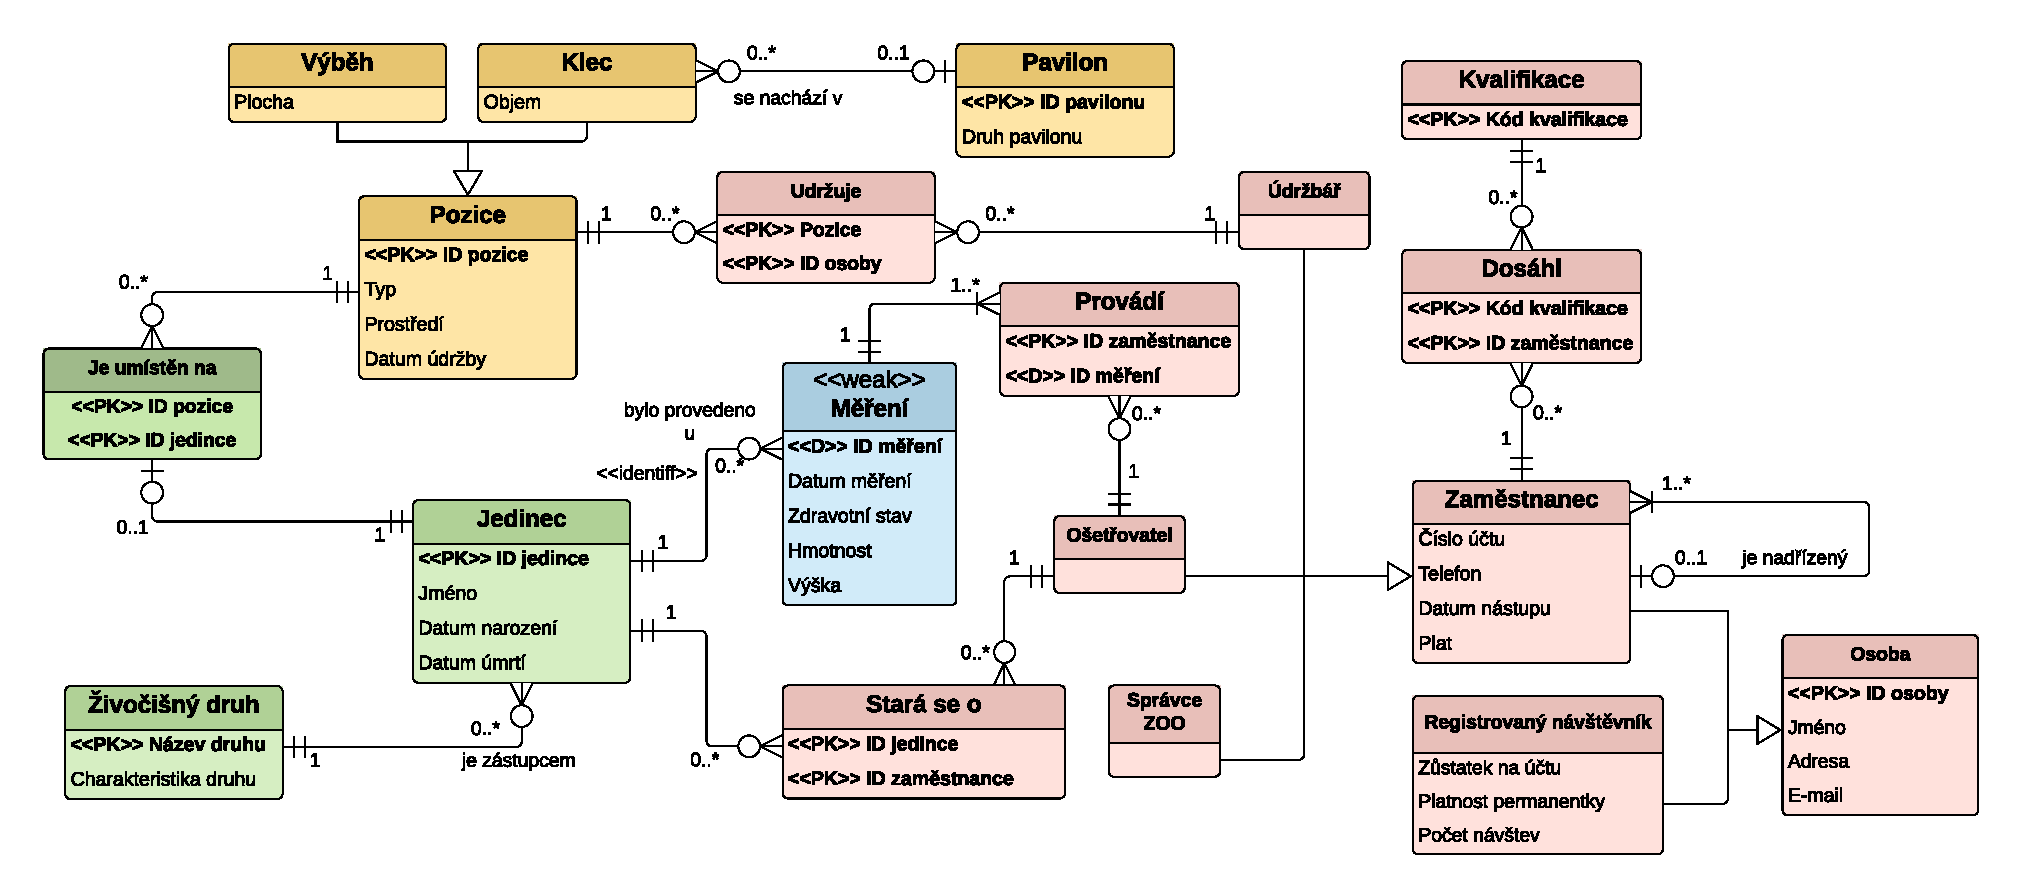
\includegraphics[scale=0.75, center]{fig/ERD_ZOO.pdf}
\vfill
\end{landscape}

\newpage
Klec se může nacházet pouze v určitém pavilonu, nebo také volně mimo pavilon. Výběh pak nikdy nepřísluší k určitému pavilonu. O~oboje se stará údržbář, tedy udržuje pozici, která generalizuje výběh a klec. Na pozici je umístěn jedinec příslušící jednomu živočišnému druhu. U~jedince je možné provádět měření (bez jedince nemá smysl vést údaj o neexistujícím měření, proto je měření modelováno jako slabá entitní množina). Měření může být provedeno maximálně jednou za den, což umožňuje procházet jeho historii. Měření provádí ošetřovatel. Společně se správcem ZOO a údržbářem jsou tyto tři typy zaměstnanců rovnocenní, pokud jde o atributy, proto jejich atributy sjednocuje entitní množina zaměstnanec, která je specializací entitní množiny osoba. O jednotlivých zaměstnancích také vedeme záznam o jejich kvalifikacích opravňujících zaměstnance vykonávat jednotlivé úkony v ZOO. Specializace zaměstnanců zde není vzhledem k atributům nutná, ale pro lepší vizualizaci vztahů mezi entitami jsme jednotlivé typy zaměstnanců explicitně oddělili. Specializací entitní množiny osoba je také registrovaný návštěvník, který si do ZOO může koupit permanentku a vložit peníze pro utracení za doplňkové služby ZOO (jídlo, dárkové předměty aj.).